%%%%%%%%%%%%%%%%%%%%%%%%%%%%%%%%%%%%%%%%%
% baposter Landscape Poster
% LaTeX Template
% Version 1.0 (11/06/13)
%
% baposter Class Created by:
% Brian Amberg (baposter@brian-amberg.de)
%
% This template has been downloaded from:
% http://www.LaTeXTemplates.com
%
% License:
% CC BY-NC-SA 3.0 (http://creativecommons.org/licenses/by-nc-sa/3.0/)
%
%%%%%%%%%%%%%%%%%%%%%%%%%%%%%%%%%%%%%%%%%

%----------------------------------------------------------------------------------------
%	PACKAGES AND OTHER DOCUMENT CONFIGURATIONS
%----------------------------------------------------------------------------------------

\documentclass[landscape,a0paper,fontscale=0.285]{baposter} % Adjust the font scale/size here

\usepackage{graphicx} % Required for including images
\graphicspath{{figures/}} % Directory in which figures are stored

\usepackage{amsmath} % For typesetting math
\usepackage{amssymb} % Adds new symbols to be used in math mode

\usepackage{booktabs} % Top and bottom rules for tables
\usepackage{enumitem} % Used to reduce itemize/enumerate spacing
\usepackage{palatino} % Use the Palatino font
\usepackage[font=small,labelfont=bf]{caption} % Required for specifying captions to tables and figures
\usepackage{hyperref}
\usepackage{caption}
\usepackage{multicol} % Required for multiple columns
\setlength{\columnsep}{1.5em} % Slightly increase the space between columns
\setlength{\columnseprule}{0mm} % No horizontal rule between columns
\usepackage{multirow}% http://ctan.org/pkg/multirow
\usepackage{hhline}% http://ctan.org/pkg/hhline
\usepackage{tikz} % Required for flow chart
\usepackage{amsmath}
\usepackage{graphicx}
\usepackage{bm}
\usetikzlibrary{shapes,arrows} % Tikz libraries required for the flow chart in the template

\newcommand{\compresslist}{ % Define a command to reduce spacing within itemize/enumerate environments, this is used right after \begin{itemize} or \begin{enumerate}
\setlength{\itemsep}{1pt}
\setlength{\parskip}{0pt}
\setlength{\parsep}{0pt}
}

\definecolor{lightblue}{rgb}{0.53,0.81,0.98} % Defines the color used for content box headers
\DeclareMathOperator*{\argmin}{arg\,min}

\begin{document}

\begin{poster}
{
headerborder=closed, % Adds a border around the header of content boxes
colspacing=1em, % Column spacing
bgColorOne=white, % Background color for the gradient on the left side of the poster
bgColorTwo=white, % Background color for the gradient on the right side of the poster
borderColor=lightblue, % Border color
headerColorOne=white, % Background color for the header in the content boxes (left side)
headerColorTwo=lightblue, % Background color for the header in the content boxes (right side)
headerFontColor=black, % Text color for the header text in the content boxes
boxColorOne=white, % Background color of the content boxes
textborder=roundedleft, % Format of the border around content boxes, can be: none, bars, coils, triangles, rectangle, rounded, roundedsmall, roundedright or faded
eyecatcher=true, % Set to false for ignoring the left logo in the title and move the title left
headerheight=0.1\textheight, % Height of the header
headershape=roundedright, % Specify the rounded corner in the content box headers, can be: rectangle, small-rounded, roundedright, roundedleft or rounded
headerfont=\Large\bf\textsc, % Large, bold and sans serif font in the headers of content boxes
%textfont={\setlength{\parindent}{1.5em}}, % Uncomment for paragraph indentation
linewidth=2pt % Width of the border lines around content boxes
}
%----------------------------------------------------------------------------------------
%	TITLE SECTION 
%----------------------------------------------------------------------------------------
%
{
\includegraphics[height=5em]{usc_logo.png}} % First university/lab logo on the left
{\bf\textsc{\huge ESTHER: Extremely Simple Image Translation Through Self-Regularization}\vspace{.1em}} % Poster title
{\textsc{Chao ``Harry'' Yang*, Taehwan Kim$^\dagger$, Ruizhe Wang$^\dagger$, Hao Peng$^\dagger$ and C.-C. Jay Kuo* \hspace{12pt} \parbox{0.3\textwidth}{\small *University of Southern California\\$^\dagger$OBEN Inc.}}} % Author names and institution
{
\includegraphics[height=5em]{oben_logo.png}} 
%----------------------------------------------------------------------------------------
%	OBJECTIVES
%----------------------------------------------------------------------------------------

\headerbox{Overview}{name=objectives,column=0,span=1, row=0}{
\begin{minipage}[t]{1\linewidth}
\begin{center}
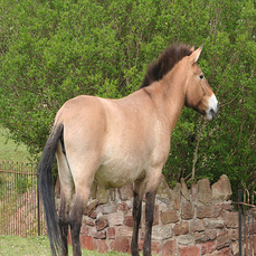
\includegraphics[width=.35\columnwidth]{figures/n02381460_2100_real_A.png}

\includegraphics[width=.2\columnwidth]{figures/arrow2.png}
\includegraphics[width=.35\columnwidth]{figures/n02381460_2100_fake_B.jpg}
\end{center}
\end{minipage}
\noindent\textbf{Problem: }\emph{Unpaired image translation between two domains}, where the goal is to learn the mapping from an input image in the source domain to an output image in the target domain. \\
\noindent\textbf{Challenge: } An ill-posed task (no paired data)! \\
\noindent\textbf{Method: }An extremely simple yet effective image translation approach, which consists of a \emph{single generator} and is trained with a \emph{self-regularization term} and an \emph{adversarial term}. \\
\noindent\textbf{Results: }Our model achieves better performance than other methods on a broad range of tasks and applications. 
\vspace{0.3em} % When there are two boxes, some whitespace may need to be added if the one on the right has more content
}


\headerbox{Related Works}{name=algorithm,column=0,span=1, 
 below=objectives}{
 %\vspace{0.3cm}
\noindent\textbf{CycleGAN:} relies on ``laziness'' of neural network and cycle-consistency to ensure 1-1 mapping.\\
\begin{minipage}[t]{1\linewidth}
\begin{center}
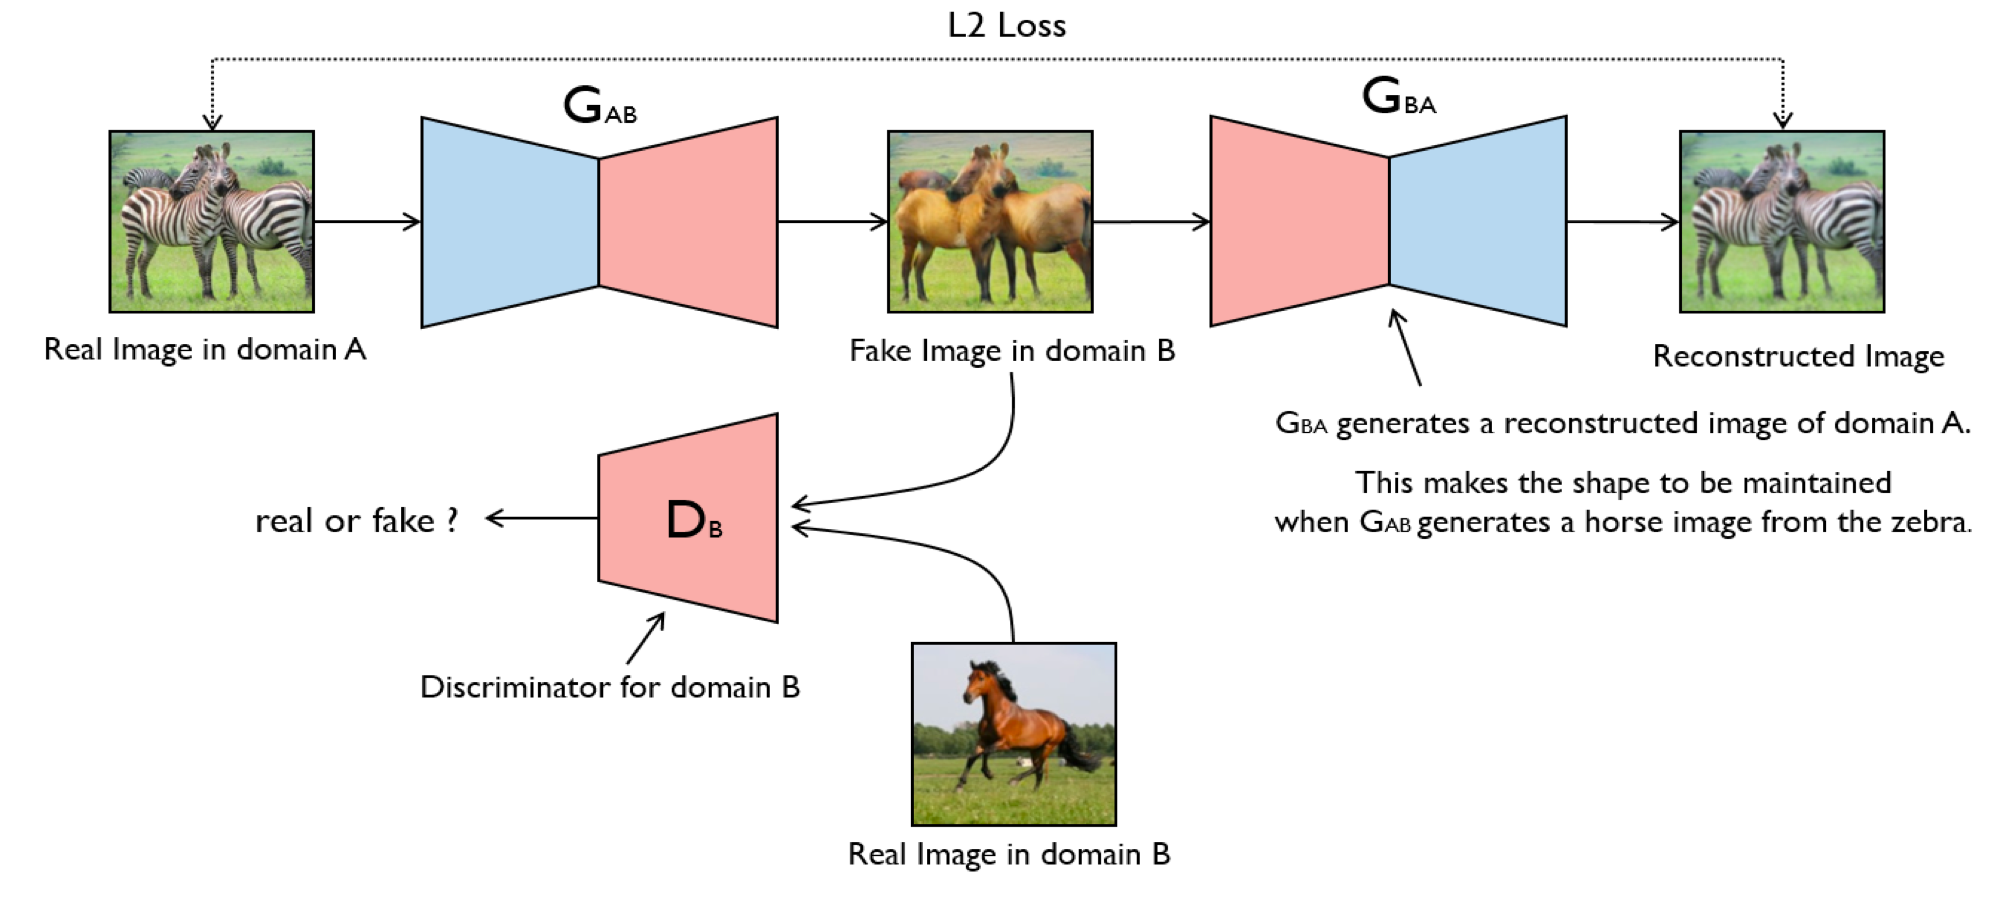
\includegraphics[width=1\columnwidth]{figures/cyclegan.png}
\end{center}
\end{minipage}
\noindent\textbf{UNIT:} relies on shared latent space and cycle-consistency.\\
\begin{minipage}[t]{1\linewidth}
\begin{center}
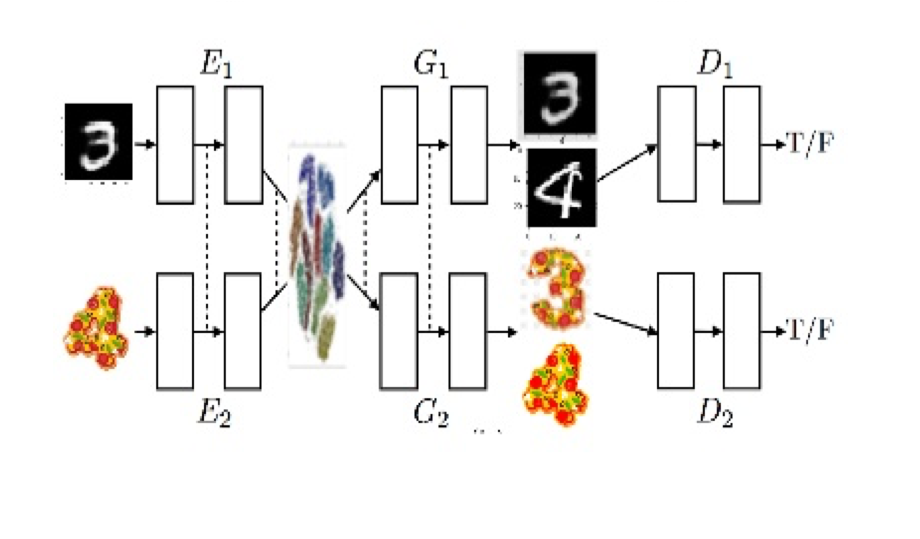
\includegraphics[width=1\columnwidth]{figures/unit.png}
\end{center}
\end{minipage}
%\vspace{0.1cm}
}

%----------------------------------------------------------------------------------------
%	INTRODUCTION
%----------------------------------------------------------------------------------------

\headerbox{Our Model}{name=content,column=1,span=2, row=0}{
\begin{minipage}{1\linewidth}
\begin{minipage}[t]{1\linewidth}
\begin{center}
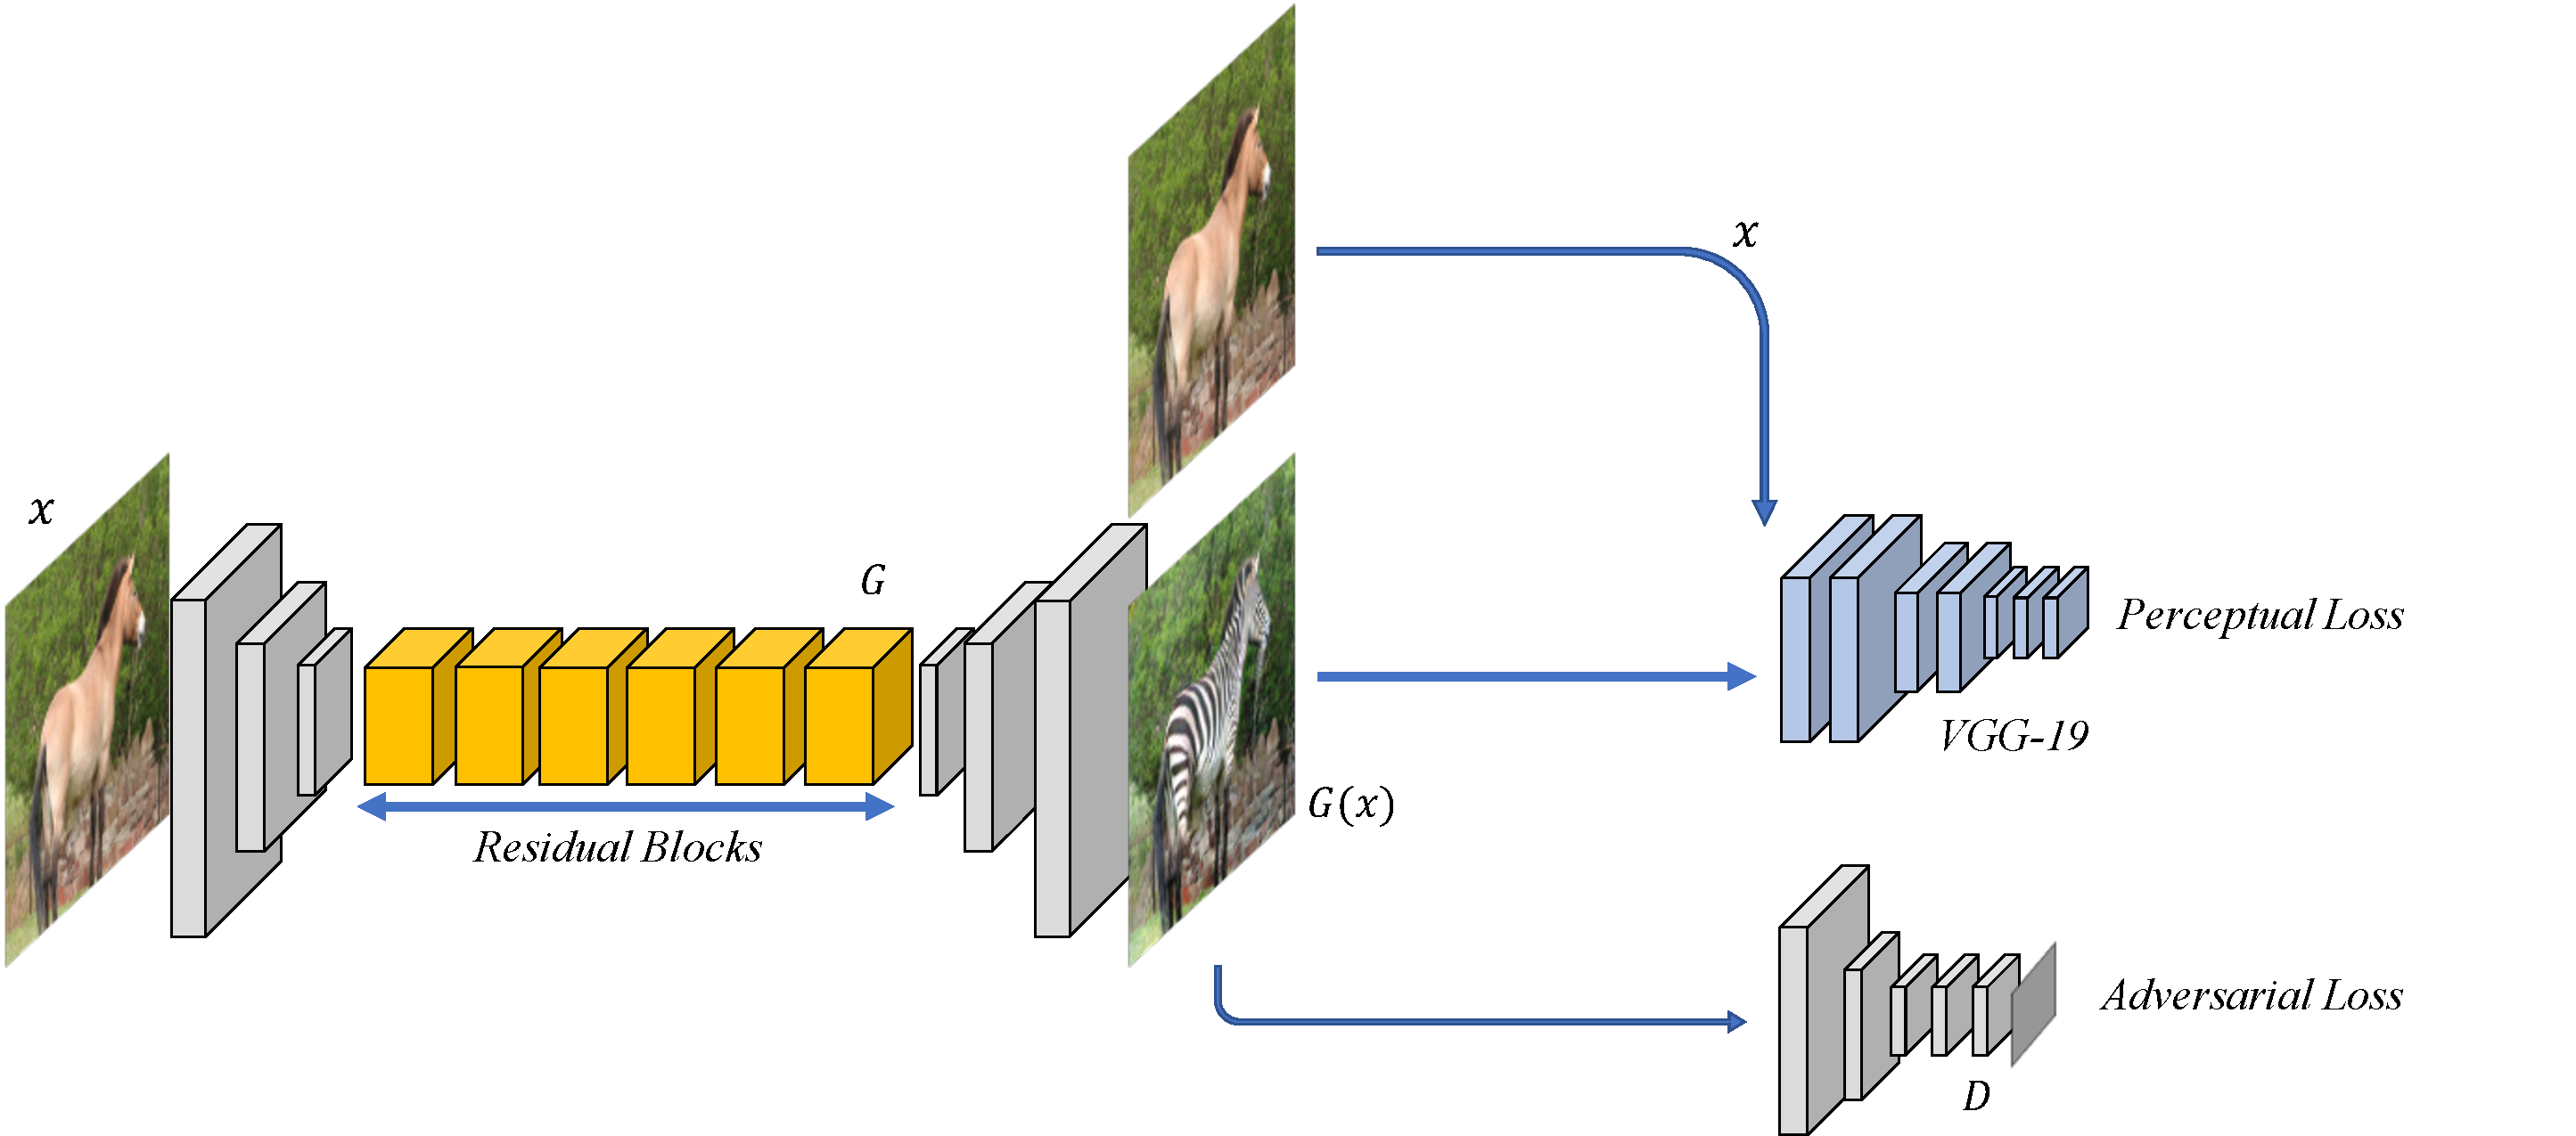
\includegraphics[width=1\columnwidth]{figures/arch2.pdf}
\end{center}
\end{minipage}
Our model consists of a single generator $G$ that maps an image from one domain to another domain. We train $G$ using the self-regularization perceptual loss and the adversarial loss:
\begin{equation*}
\mathcal{L}_{G}(\theta) = \ell_{adv}(G_\theta(x),Y) + \lambda \ell_{reg}(x, G_\theta(x)).
\end{equation*}
\end{minipage}
}

\headerbox{Training Details}{name=texture,column=1,span=1, below=content}{
\vspace{0.5cm}
\noindent\textbf{Training Losses:}
\begin{itemize}[leftmargin=*]
\item Image domain adversarial loss (with PatchGAN):
\begin{eqnarray*}
&& \ell_{adv}(G_\theta(x),Y) = \\ 
&&E_{y\sim Y}[\log D(y)] + E_{x\sim X}[\log(1-D(G(x)))].
\end{eqnarray*}
\item The self-regularization loss (with Perceptual Loss):
\begin{eqnarray*}
&&\ell_{reg}(y',x)= \sum\limits_{l=1}^3\frac{1}{H_lW_l} \\
&&\sum\limits_{h,w}(\parallel w_l^T\circ (\hat{F}(x)^l_{hw}-\hat{F}(y')_{hw}^l)\parallel_2^2).
\end{eqnarray*}
\end{itemize}
Notes: we use VGG-19 pre-trained on ImageNet as $F$. We obtained the best results by using the first three layers of VGG-19, which preserves the low-level traits of the input during translation. 
\vspace{0.5cm}
}


\headerbox{\small Training Details}{name=drop_adversarial,column=2,span=1, below=content}{ 
\noindent\textbf{Adaptive weight induction :}\\
\emph{Problem: } How to select $\lambda$, the weight of the self-regularization term relative to the image adversarial term? \\
\emph{Existing approach: } Empirically and fixed (CycleGAN, UNIT, etc.).\\
\emph{Our approach: } Adaptive and dynamic.\\
we start by setting $\lambda=0$, then we gradually increase $\lambda$, until the adversarial loss increases above some threshold $\ell_{adv}^t$.
}

\headerbox{\small Analysis}{name=comparison,column=2,span=1, below=drop_adversarial}{
Effects of using different layers as feature extractors:\\
\begin{minipage}[t]{1\linewidth}
\begin{center}
\centering
\small
\setlength\tabcolsep{1pt}
\begin{tabular}{cccc}
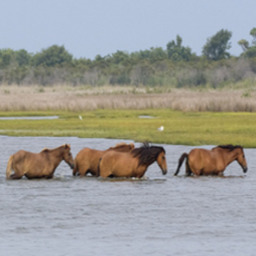
\includegraphics[width=.24\textwidth]{figures/ablation/input.jpg}&
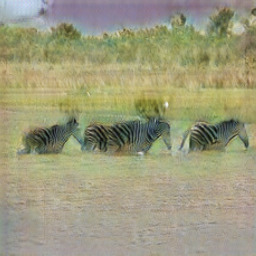
\includegraphics[width=.24\textwidth]{figures/ablation/0_1.jpg}&
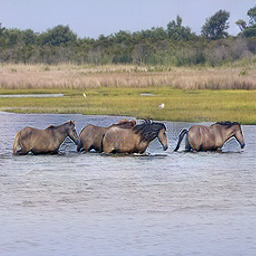
\includegraphics[width=.24\textwidth]{figures/ablation/3_4.jpg}&
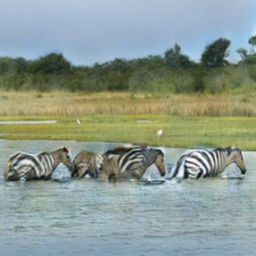
\includegraphics[width=.24\textwidth]{figures/ablation/0_2.jpg} \\
(a) & (b) & (c) & (d) \\
\end{tabular}
\end{center}
\end{minipage}
(a) input. (b) using the first two layers of VGG. (c) using the last two layers of VGG. (d) using the first three layers of VGG.
}

\headerbox{\small Visual Comparisons}{name=imagenet,column=3,span=1, row=0}{ 
\begin{minipage}{1\linewidth}
\setlength\tabcolsep{1.5pt}
\centering
\tiny
\begin{tabular}{cccc}
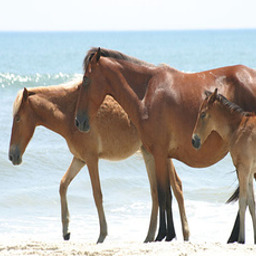
\includegraphics[width=.24\textwidth]{figures/horse2zebra/n02381460_120_real_A.jpg}&
  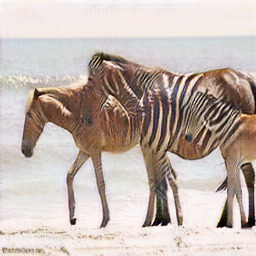
\includegraphics[width=.24\textwidth]{figures/horse2zebra/n02381460_120_fake_B-1.jpg}&
  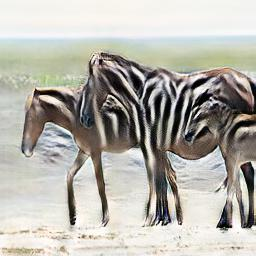
\includegraphics[width=.24\textwidth]{figures/UNIT/n02381460_120.jpg}&
  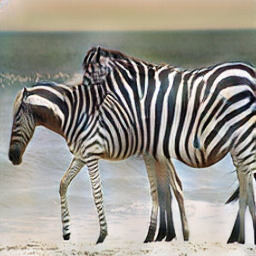
\includegraphics[width=.24\textwidth]{figures/horse2zebra/n02381460_120_fake_B.jpg} \\
 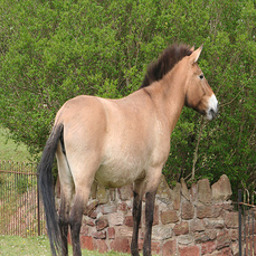
\includegraphics[width=.24\textwidth]{figures/horse2zebra/n02381460_2100_real_A.jpg}&
  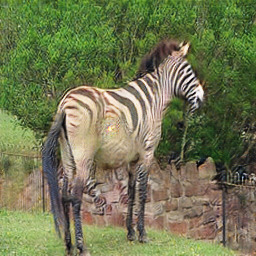
\includegraphics[width=.24\textwidth]{figures/horse2zebra/n02381460_2100_fake_B-1.jpg}&
  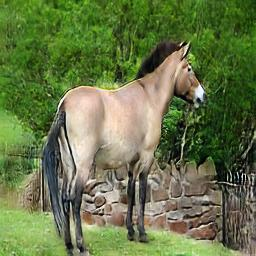
\includegraphics[width=.24\textwidth]{figures/UNIT/n02381460_2100.jpg}&
  \includegraphics[width=.24\textwidth]{figures/horse2zebra/n02381460_2100_fake_B.jpg} \\
    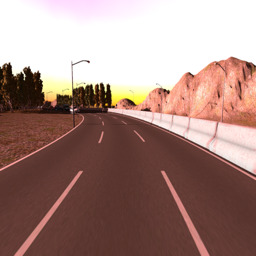
\includegraphics[width=.24\textwidth]{figures/dawn2night/001104_real_A.jpg}&
  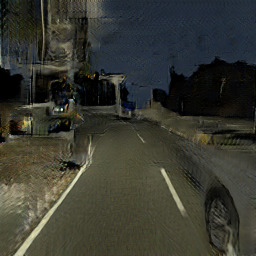
\includegraphics[width=.24\textwidth]{figures/dawn2night/001104_fake_B-1.jpg}&
  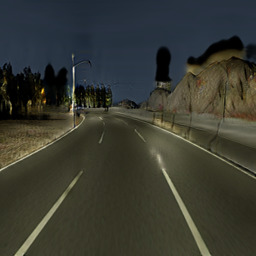
\includegraphics[width=.24\textwidth]{figures/UNIT/001104.jpg}&
  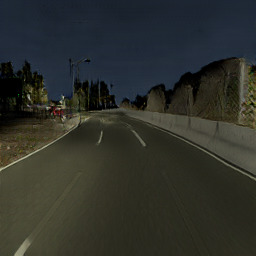
\includegraphics[width=.24\textwidth]{figures/dawn2night/001104_fake_B.jpg} \\
      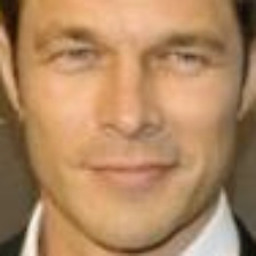
\includegraphics[width=.24\textwidth]{figures/smile/000033_real_A2.jpg}&
  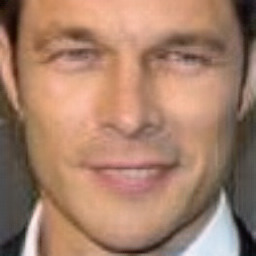
\includegraphics[width=.24\textwidth]{figures/smile/000033_fake_B-1.jpg}&
  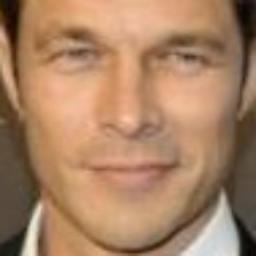
\includegraphics[width=.24\textwidth]{figures/UNIT/output.jpg}&
  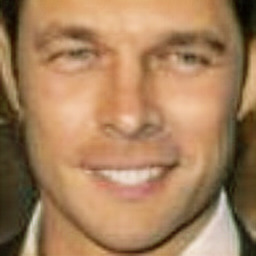
\includegraphics[width=.24\textwidth]{figures/smile/000033_fake_B.jpg} \\
   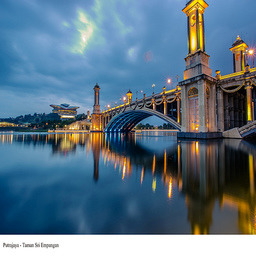
\includegraphics[width=.24\textwidth]{figures/vangoh/input.jpg}&
  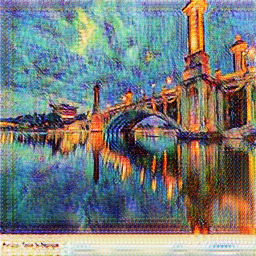
\includegraphics[width=.24\textwidth]{figures/vangoh/cycle.jpg}&
  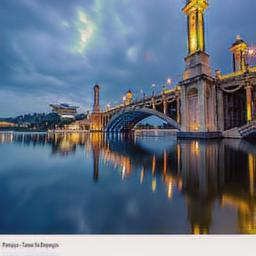
\includegraphics[width=.24\textwidth]{figures/UNIT/vangoh.jpg}&
  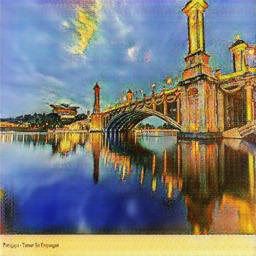
\includegraphics[width=.24\textwidth]{figures/vangoh/ours.jpg} \\
   (a) Input & (b) CycleGAN  & (c) {UNIT} & (d) Ours  \\
\end{tabular}
%\caption{The effect of texture weight $\alpha$. }\label{alpha}
\end{minipage}
}

\headerbox{\small More Results}{name=paris,column=3,span=1, below=imagenet}{ 
\begin{minipage}{1\linewidth}
\setlength\tabcolsep{1.5pt}
\centering
\tiny
\begin{tabular}{cccc}
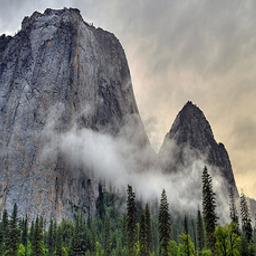
\includegraphics[width=.24\textwidth]{figures/others/summer_yose.jpg}&
  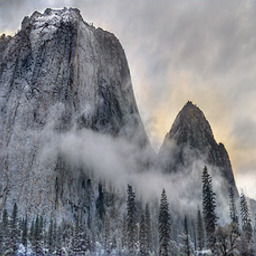
\includegraphics[width=.24\textwidth]{figures/others/winter_yose.jpg}&
  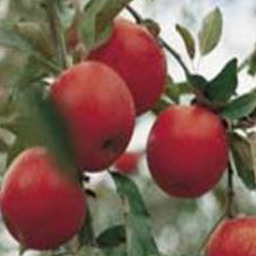
\includegraphics[width=.24\textwidth]{figures/others/apple.jpg}&
  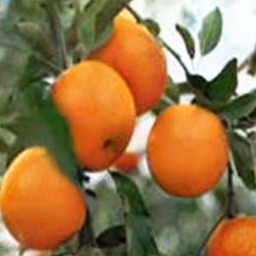
\includegraphics[width=.24\textwidth]{figures/others/orange.jpg}\\
  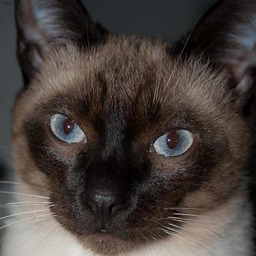
\includegraphics[width=.24\textwidth]{figures/others/cat_1036_real_A.jpg}&
   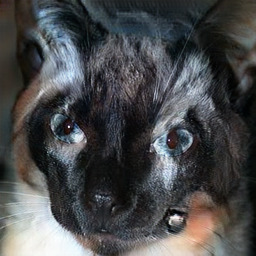
\includegraphics[width=.24\textwidth]{figures/others/cat_1036_fake_B.jpg} &
   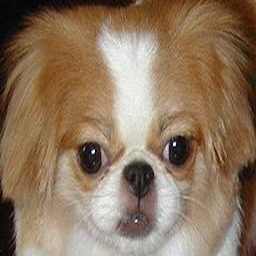
\includegraphics[width=.24\textwidth]{figures/others/dog_1035_real_A.jpg}&
  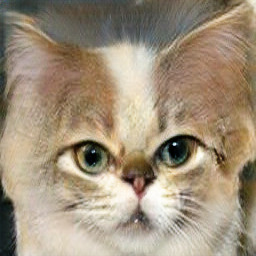
\includegraphics[width=.24\textwidth]{figures/others/dog_1035_fake_B.jpg}\\
  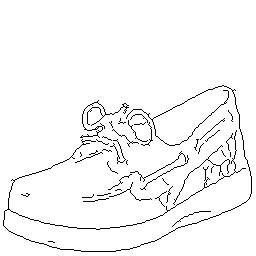
\includegraphics[width=.24\textwidth]{figures/others/1003_real_A.jpg}&
  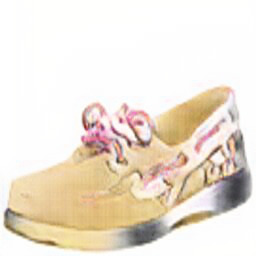
\includegraphics[width=.24\textwidth]{figures/others/1003_fake_B.jpg}&
 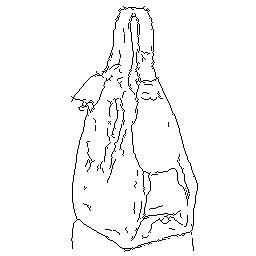
\includegraphics[width=.24\textwidth]{figures/others/100008_real_A.jpg}&
  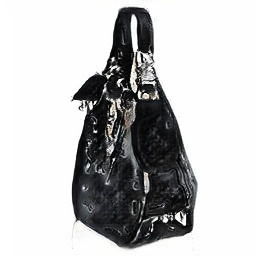
\includegraphics[width=.24\textwidth]{figures/others/100008_fake_B.jpg} \\
  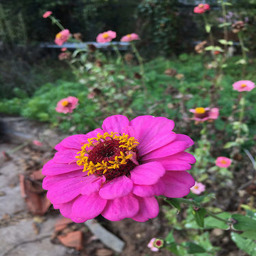
\includegraphics[width=.24\textwidth]{figures/others/flower1.jpg}&
  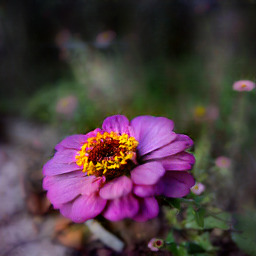
\includegraphics[width=.24\textwidth]{figures/others/flower2.jpg}&
 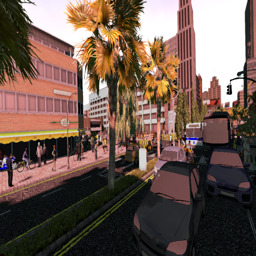
\includegraphics[width=.24\textwidth]{figures/others/epoch020_real_A.jpg}&
  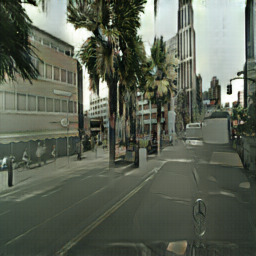
\includegraphics[width=.24\textwidth]{figures/others/epoch020_fake_B.jpg}\\

\end{tabular}
%\caption{The effect of texture weight $\alpha$. }\label{alpha}
\end{minipage}
}
\vspace{0.8em}
\headerbox{}%
{name=foottext, column=3, span=1, above=bottom,%
 textborder=none,headerborder=none,boxheaderheight=0pt}{
 Please \textbf{attend} to \url{https://arxiv.org/abs/1806.06195} for extended version!}

%----------------------------------------------------------------------------------------


\end{poster}

\end{document}